\subsubsection{Detaillierte Implementation}

Eine Übersicht der einzelnen Komponenten mit ihren genauen Zusammenhängen wird in Abbildung~\ref{asset:Capacitor-NodeJS:Implementation} dargestellt.

\begin{figure}[H]
    \centering
    \vspace{1em}
    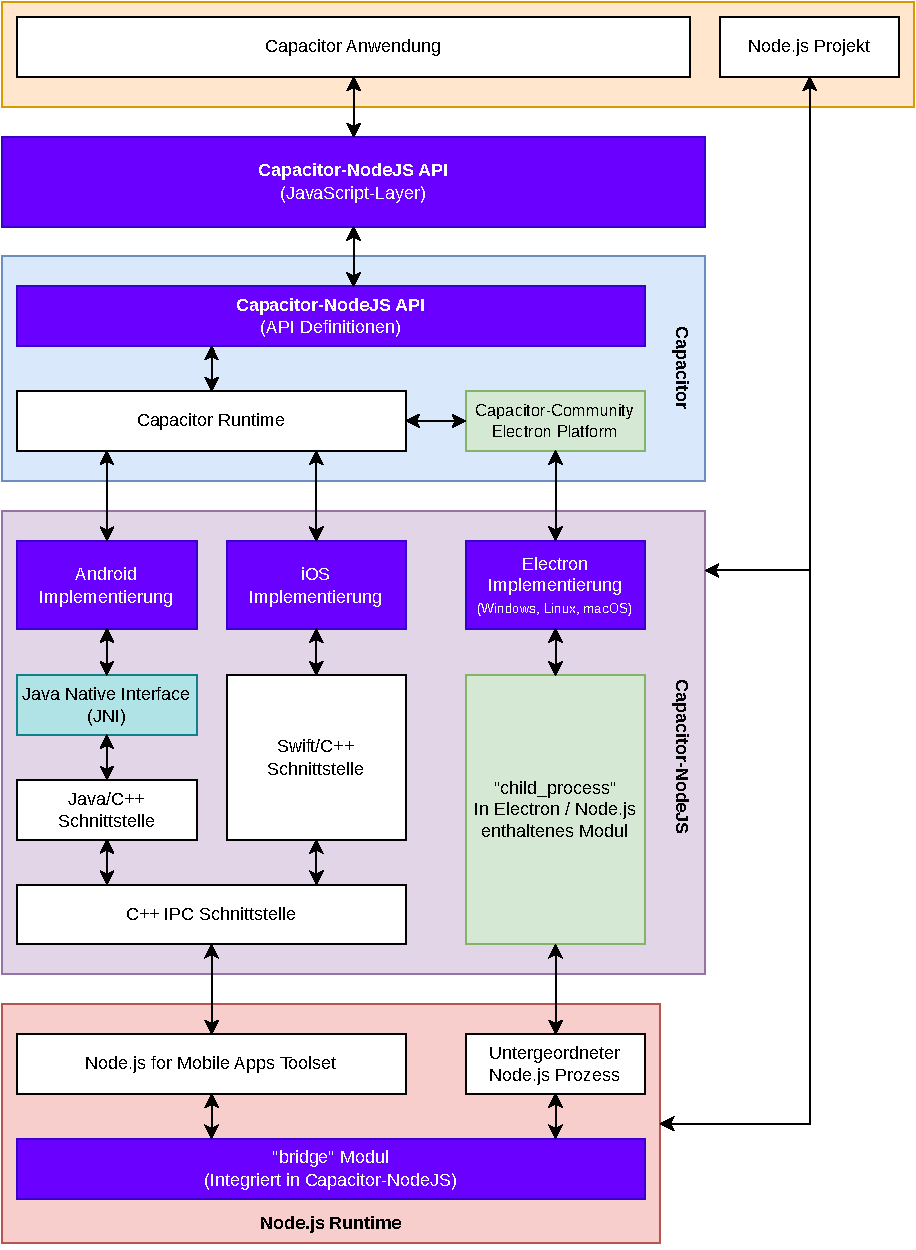
\includegraphics[width=\textwidth]{assets/02_Capacitor-NodeJS/04_Implementation.drawio.pdf}
    \caption[Capacitor-NodeJS / Implementierung]{Implementierung des Capacitor-NodeJS Plugins}
    \label{asset:Capacitor-NodeJS:Implementation}
\end{figure}

\newpage

\paragraph{Plugin API}

Das Capacitor-NodeJS Plugin erweitert seine \ac{api} um einen zusätzlichen JavaScript"=Layer, der zusätzliche nicht-native Funktionen implementiert.
Damit wird das das Entfernen bestimmter oder aller Event-Listener ermöglicht.

\paragraph{Implementierungen}

Um die Implementierung des Plugins auf allen Plattformen übersichtlich und wartungsfreundlich zu gestalten, sind sie in ihrer Struktur sehr ähnlich.
Sie bestehen jeweils aus zwei Teilen:

\begin{enumerate}
    \item 
    Der erste Teil wird von der Capacitor Runtime aufgerufen.
    Er implementiert die \acs{api}-Struktur und wertet die Parameter der Methoden aus.
    \item 
    Der zweite Teil implementiert die tatsächlichen Funktionen,
    wie das Starten der Node.js Runtime sowie das Senden und Empfangen von Nachrichten zwischen den Prozessen.
\end{enumerate}

Um eine Node.js Runtime auf Desktop"=Plattformen (Windows, Linux und macOS) zu starten, wird bei der Electron Implementierung das von Electron bzw.\ Node.js bereitgestellte Modul \code{child_process} verwendet.
\cite{electron:docs}

Bei der Android Implementierung müssen für das Starten der Runtime jedoch mehrere Punkte beachtet werden:

\begin{itemize}
    \item
    Android Anwendungen sind wie Archive aufgebaut.
    Das bedeutet, dass sie aus einer Reihe von Dateien bestehen, die in einem komprimierten Format gespeichert sind.
    Daher muss das Node.js Projekt von der Anwendung in das Android Dateisystem kopiert werden, damit die Node.js Runtime darauf zugreifen kann.
    \cite{nodejs-mobile:docs}

    \item 
    Um von der Implementierung auf die nativen Binärdateien der Node.js Runtime zuzugreifen, ist unter Android und iOS ein C++ Code als Schnittstelle erforderlich.
    Für die Integration des nativen Codes unter Android ist zusätzlich das \ac{ndk} erforderlich.
    Der verwendete Code für diese Schnittstelle stammt aus der Dokumentation des Node.js for Mobile Apps Toolsets.
    \cite{nodejs-mobile:docs}
\end{itemize}

\newpage

\paragraph{Interprozesskommunikation}

Die Kommunikation zwischen der Node.js Runtime, der Plugin Implementierung und der Capacitor Anwendung wird unter Windows, Linux und MacOS bzw.\ in der Electron Implementierung des Plugins hauptsächlich durch das \code{child_process} Modul verwaltet.
\cite{electron:docs}

Unter Android und iOS erfordert diese Kommunikation erneut nativen C++ Code.
Dieser Code dient als native \acp{ipc} Schnittstelle und ist von der Android Implementierung des Plugins aufrufbar und über die Node-API auch für JavaScript-Code in der Node.js Runtime zugänglich.
Dadurch kann eine Art Event-Emitter realisiert werden.
\cite{nodejs-mobile-cordova, nodejs}

Der verwendete Code für diese \ac{ipc} Schnittstelle stammt aus dem Node.js for Mobile Apps Cordova Plugin.
\cite{nodejs-mobile-cordova}

\vspace{1em}

\begin{figure}[H]
    \centering
    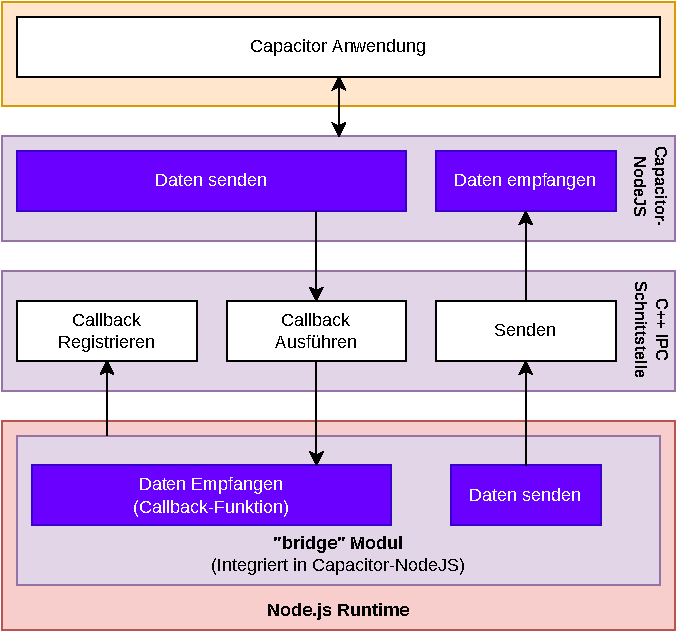
\includegraphics[width=0.8\textwidth]{assets/02_Capacitor-NodeJS/03_Interprozesskommunikation.drawio.pdf}
    \caption[Capacitor-NodeJS / Interprozesskommunikation]{Interprozesskommunikation zwischen der Capacitor Anwendung, dem Capacitor-NodeJS Plugin und der Node.js Runtime.}
\end{figure}

\vspace{-1em}

Um Daten von der Capacitor Anwendung zu empfangen, registriert ein JavaScript-Code aus der Node.js Runtime eine Callback-Funktion in der nativen \ac{ipc} Schnittstelle.
Eine Callback-Funktion ist eine Funktion, die als Parameter an eine andere Funktion übergeben wird.
Das Capacitor-NodeJS Plugin kann dann über die native Schnittstelle die Callback-Funktion aufrufen und Nutzdaten übergeben.

Um Daten an die Capacitor Anwendung zu senden, ruft ein JavaScript-Code aus der Node.js Runtime eine Funktion in der nativen Schnittstelle auf und übergibt die Nutzdaten.
Die Funktion in der Schnittstelle leitet die Daten schließlich an die Android Implementierung des Plugins weiter.

Unter Android können Nutzdaten nur als primitive Datentypen übergeben werden, daher müssen diese Daten serialisiert und deserialisiert werden.
Für die Serialisierung wurde das \ac{json} Datenformat verwendet.

Um auch in der Node.js Runtime eine Benutzerfreundliche \ac{api} zur Kommunikation mit der Capacitor Anwendung bereitzustellen, wurde ein \code{bridge} Modul erstellt, welches den JavaScript-Code für die Handhabung der Kommunikation sowie für die Serialisierung und Deserialisierung beinhaltet.
Es erweitert die Node.js Event-Emitter Klasse, um die Kompatibilität mit vorhandenen Node.js Projekten zu verbessern.
Unter Android kommuniziert das Modul wie oben beschrieben mit der nativen \ac{ipc} Schnittstelle
Unter Windows, Linux und macOS kommuniziert es über das \code{child_process} Modul von Node.js.
Das \code{bridge} Modul wird automatisch in der Node.js Runtime geladen, so dass Benutzer keine zusätzlichen Schritte ausführen müssen.

Um das automatische Laden zu ermöglichen, wird beim Start der Runtime die Umgebungsvariable \code{NODE_PATH} gesetzt.
Diese Umgebungsvariable enthält eine Liste von Pfaden, welche die Node.js Runtime nach Modulen durchsucht.
Gefundene Module werden dann für das Node.js Projekt bereit gestellt.
\cite{nodejs-mobile:docs, nodejs}
